\newpage\section{Vapnik-Chevronenkis Theory}
In the following section, we will review a notion for measuring complexity of function class called \textbf{VC dimension}. Later on in this note, we will show that VC dimension is an upper-bound for the \textbf{Rademacher Complexity}.

\subsection{VC Dimension}
\begin{definition}[Restriction ($N_\mathcal{H}$)]
    Let $\Hf \in \{0,1\}^\X$ be a set of classifiers. The \textbf{restriction} of $\Hf$ to a finite subset $C\subset\X$ where $|C| = n$ is the set of binary vectors defined by:
    \begin{align*}
        \boxed{
        N_\Hf(C) = \bigCurl{
            (h(x_1), \dots, h(x_n)) : h\in\Hf, x_i \in C
        } 
        }
    \end{align*}

    \noindent Clearly, we have $|N_\Hf(C)| \le 2^n$ (cardinality of powerset of $C$).
\end{definition}

\begin{definition}[Shattering Coefficient ($S_\Hf$)]
    The $n^{th}$ \textbf{Shattering coefficient} (sometimes called the \textbf{Growth function}) is defined as:
    \begin{align*}
        \boxed{S_\Hf(n) = \sup_{C\subset\X; |C|=n} \bigAbs{N_\Hf (C)}}
    \end{align*}

    \noindent Hence, we have:
    \begin{align*}
        |N_\Hf(C)| \le S_\Hf(n) \le 2^n, \ \forall C \subset \X
    \end{align*}

    \noindent Intuitively, the $n^{th}$ shattering coefficient is the size of the largest $n$-element restriction of $\Hf$. It measures the \textbf{richness} of $\Hf$.

    \noindent\newline If $S_\Hf(n)=2^n$. Then $\exists C\subset\X, |C|=n$ such that $\bigAbs{N_\Hf(C)}=2^n$. We then say that $\Hf$ \textbf{shatters the points in} $C$.
\end{definition}

\begin{definition}[VC-dimension ($V_\Hf$)]
    The \textbf{VC dimension} of $\Hf$ is defined as:
    \begin{align*}
        \boxed{V_\Hf = \sup\bigCurl{
            n : S_\Hf (n) = 2^n
        }=\sup_{C\subset \X}\bigCurl{
            |C| : \Hf \text{ shatters } C
        }}
    \end{align*}

    \noindent If $S_\Hf(n)=2^n, \forall n \ge 1$ then $V_\Hf=\infty$.  
\end{definition}

\noindent\textbf{Remark} : Note that when $|\Hf| < \infty$, we have:
\begin{align*}
    |N_\Hf(C)| &= \bigAbs{
        \{(h(x_1), \dots, h(x_n)) : h\in\Hf, x_i \in C\}
    } \le |\Hf| \\
    \implies S_\Hf(n) &\le |\Hf| \\
    \implies V_\Hf &\le \log_2|\Hf|
\end{align*}


\noindent \textbf{Remark} : To show that $V_\Hf=n$, we must show that there exists at least $n$ points $x_1, \dots, x_n$ shattered by $\Hf$ and no set of $n+1$ points can be shattered by $\Hf$. 

\noindent\newline \textbf{Remark} : From the above definitions, we can understand $N_\Hf, S_\Hf$ and $V_\Hf$ as followed:
\begin{itemize}
    \item $N_\Hf(C)$ : Number of ways to assign labels to $C\subset \X$ of size $n\ge1$.
    \item $S_\Hf(n)$ : Maximum number of ways to assign labels to subsets of size $n\ge1$.
    \item $V_\Hf$ : Maximum subset size $n\ge1$ such that we have $2^n$ ways to assign labels (fully labelled).
\end{itemize}



\subsection{Sauer's Lemma}
\begin{theorem}{Sauer's Lemma}{sauer_lemma}
    This is a bound on the shatter coefficient. Let $d=V_\Hf\le\infty$. For all $n\ge1$, we have:
    \begin{align*}
        S_\Hf(n) \le \sum_{k = 0}^d \begin{pmatrix}
            n \\ k
        \end{pmatrix}
    \end{align*}
\end{theorem}

\begin{proof*}[Theorem \ref{thm:sauer_lemma}, cited \cite{course:machine_learning_theory}]
    Given a function class $\Hf$ and a subset $C\subset\X$. For brevity, denote the restriction of $\Hf$ to $C$ as:
    \begin{align*}
        N_\Hf(C) = \Hf_C
    \end{align*}

    \noindent To prove the above theorem, we prove a stronger result: For all subset $C\subset\X$ where $|C|=n$, we have
    \begin{align*}
        |\Hf_C| \le \bigAbs{
            \bigCurl{
                B \subset C : \Hf \text{ shatters } B
            }
        } \le \sum_{k=0}^d \begin{pmatrix}
            n\\k
        \end{pmatrix}
    \end{align*}

    \noindent The second inequality holds because no set with size larger than $d$ is shattered by $\Hf$. To prove that the first inequality holds for subsets of any size $n\ge1$, we prove by induction:

    \begin{itemize}
        \item \textbf{Base case} : Let $n=1$. Hence, we have $C=\{x\}$ for $x\in\X$. Denote that:
        \begin{align*}
            \Phi_C = \bigCurl{
                B \subset C : \Hf \text{ shatters } B
            }
        \end{align*}
        \noindent We have:
        
        \[
            \begin{cases}
                \Hf \text{ shatters } C &\implies \Hf_C = \{0,1\} , \Phi_C = \{\emptyset, C\}
                \\ \\
                \Hf \text{ not shatter } C &\implies \Hf_C = \{0\} \text{ or } \{1\} , \Phi_C = \{\emptyset\}
            \end{cases}  
        \]

        \noindent For both cases, we have $|\Hf_C| = |\Phi_C|$.

        \item \textbf{Inductive case} : Assume that the first inequality holds for $n=m-1, m \ge 2$, We have to prove that it holds for $n=m$. Let $C=\{c_1, \dots, c_m\}$ and $C'=\{c_2, \dots, c_m\}$. Define the following label sets:
        \begin{align*}
            Y_0 &= \{(y_2, \dots, y_m) : (0, y_2, \dots, y_m) \in \Hf_C \vee (1, y_2, \dots, y_m) \in \Hf_C \}
            \\ \\
            Y_1 &= \{(y_2, \dots, y_m) : (0, y_2, \dots, y_m) \in \Hf_C \wedge (1, y_2, \dots, y_m) \in \Hf_C\}
        \end{align*}

        \noindent First, we notice that $Y_0 = \Hf_{C'}$. Hence, we have:
        \begin{align*}
            |Y_0| &= |\Hf_{C'}| \\
                &\le \bigAbs{
                    \bigCurl{
                        B \subset C' : \Hf \text{ shatters } B
                    }
                } \\
                &= \bigAbs{
                    \bigCurl{
                        B \subset C : c_1 \notin B, \Hf \text{ shatters } B
                    }
                }
        \end{align*}

        \noindent Next, we define the following sub-class of $\Hf$:
        \begin{align*}
            \Hf' = \biggCurl{
                h \in \Hf : \exists h' \in \Hf \text{ s.t } h'(c) = \begin{cases}
                    1 - h(c) &\text{if } c=c_1
                    \\
                    h(c) &\text{otherwise}
                \end{cases} 
            }
        \end{align*}

        \noindent Note that $Y_1 = \Hf'_{C'}$ and $\Hf'$ shatters $B\in C'$ implies $\Hf'$ shatters $B\cup\{c_1\}$ because for any $h'\in\Hf'$, there is always another function in $\Hf'$ that gives the opposite label to $c_1$. Hence, we have:
        \begin{align*}
            |Y_1| &= |\Hf'_{C'}| \\
                &\le \bigAbs{
                    \bigCurl{
                        B \subset C' : \Hf' \text{ shatters } B
                    }
                } \\
                &= \bigAbs{
                    \bigCurl{
                        B \subset C' : \Hf' \text{ shatters } B \cup \{c_1\}
                    }
                } \\
                &= \bigAbs{
                    \bigCurl{
                        B \subset C : c_1\in B, \Hf' \text{ shatters } B
                    }
                } \\
                &\le \bigAbs{
                    \bigCurl{
                        B \subset C : c_1\in B, \Hf \text{ shatters } B
                    }
                } 
        \end{align*}

        \noindent From the above, we have:
        \begin{align*}
            |\Hf_C| &= |Y_0| + |Y_1| \\
                &\le \bigAbs{
                    \bigCurl{
                        B \subset C : c_1 \notin B, \Hf \text{ shatters } B
                    }
                } + \bigAbs{
                    \bigCurl{
                        B \subset C : c_1\in B, \Hf \text{ shatters } B
                    }
                } \\
                &= \bigAbs{
                    \bigCurl{
                        B \subset C : \Hf \text{ shatters } B
                    }
                } \\
                &\le \sum_{k=0}^d \begin{pmatrix}
                    n\\k
                \end{pmatrix}
        \end{align*}

        \noindent Taking the supremum over $C\subset\X$ for both sides, we have:
        \begin{align*}
            S_\Hf(n) \le \sum_{k=0}^d \begin{pmatrix}
                n\\k
            \end{pmatrix}
        \end{align*}
    \end{itemize}
\end{proof*}

\begin{corollary}{Sauer's lemma - bound on $S_\Hf(n)$ I}{sauer_bound_on_shattering_coeff_I}
    If $d=V_\Hf < \infty$, for all $n\ge1$, we have:
    \begin{align*}
        S_\Hf(n) \le (n+1)^d
    \end{align*}
\end{corollary}

\begin{proof*}[Corollary \ref{coro:sauer_bound_on_shattering_coeff_I}]
    By Binomial theorem, we have:
    \begin{align*}
        (n+1)^d &= \sum_{k=1}^d n^k \begin{pmatrix} d \\ k \end{pmatrix} \\
        &= \sum_{k=1}^d n^k \frac{d!}{k!(d-k)!} \\
        &\ge \sum_{k=1}^d \frac{n^k}{k!} \ge \sum_{k=1}^d\frac{n!}{(n-k)!k!} = \sum_{k=1}^d \begin{pmatrix}
            n \\ k
        \end{pmatrix} \ge S_\Hf(n)
    \end{align*}
\end{proof*}

\begin{corollary}{Sauer's lemma - bound on $S_\Hf(n)$ II}{sauer_bound_on_shattering_coeff_II}
    For all $n\ge d=V_\Hf$, we have:
    \begin{align*}
        S_\Hf(n) \le \biggRound{
            \frac{ne}{d}
        }^d
    \end{align*}
\end{corollary}

\begin{proof*}[Corollary \ref{coro:sauer_bound_on_shattering_coeff_II}]
    For $\frac{d}{n} < 1$, we have:
    \begin{align*}
        \biggRound{\frac{d}{n}}^d \sum_{k=0}^d \begin{pmatrix}
            n \\ k
        \end{pmatrix} &\le \sum_{k=0}^d \biggRound{\frac{d}{n}}^k \begin{pmatrix}
            n \\ k
        \end{pmatrix} \\
        &\le \sum_{k=0}^n \biggRound{\frac{d}{n}}^k \begin{pmatrix}
            n \\ k 
        \end{pmatrix} \\
        &= \biggRound{1 + \frac{d}{n}}^n \le e^d
    \end{align*}

    \noindent Hence, we have:
    \begin{align*}
        \biggRound{\frac{en}{d}}^d \ge \sum_{k=0}^d \begin{pmatrix}
            n \\ k
        \end{pmatrix} \ge S_\Hf(n)
    \end{align*}
\end{proof*}

\begin{corollary}{Sauer's lemma - bound on $S_\Hf(n)$ III}{sauer_bound_on_shattering_coeff_III}
    If $V_\Hf=d>2$, for all $n\ge d$, we have:
    \begin{align*}
        S_\Hf(n) \le n^d
    \end{align*}
\end{corollary}

\begin{proof*}[Corollary \ref{coro:sauer_bound_on_shattering_coeff_III}]
    If $d>2$ then by corollary \ref{coro:sauer_bound_on_shattering_coeff_II}, we have:
    \begin{align*}
        \frac{e}{d} < 1 \implies S_\Hf(n) \le \biggRound{\frac{en}{d}}^d \le n^d
    \end{align*}
\end{proof*}

\subsection{VC Theorem}
\begin{theorem}{VC Theorem (for classifiers)}{udb_non_finite_h}
    For any $n\ge1$ and $\epsilon>0$, we have:
    \begin{align*}
        P\biggRound{
            \sup_{h\in\Hf} \bigAbs{
                \widehat{R_n}(h) - R(h)
            } \ge \epsilon
        } \le 8S_\Hf(n) e^{-n\epsilon^2/32}
    \end{align*}
\end{theorem}

\begin{proof*}[Theorem \ref{thm:udb_non_finite_h}]
    The proof for this theorem will be mentioned later in section \ref{sec:proof_of_vc_inequality}. For now, we will assume that it is true to prove the following corollaries.
\end{proof*}

\begin{corollary}{Convergence of Empirical Risk (VC-Theorem)}{convergence_of_emp_risk_vc}
    If $\widehat{h_n}$ is an empirical risk minimizer over $\Hf$ then:
    \begin{align*}
        P\bigRound{
            R(\widehat{h_n}) - R_\Hf^* \ge \epsilon
        } \le 8S_\Hf(n)e^{-n\epsilon^2/128}
    \end{align*}
\end{corollary}

\begin{proof*}[Corollary \ref{coro:convergence_of_emp_risk_vc}]
    We have:
    \begin{align*}
        P\bigRound{
            R(\widehat{h_n}) - R_\Hf^* \ge \epsilon
        } 
        &\le 
        P\biggRound{
            2\sup_{h\in\Hf} \bigAbs{\widehat{R_n}(h) - R(h)} \ge \epsilon
        } \\
        &= 
        P\biggRound{
            \sup_{h\in\Hf} \bigAbs{\widehat{R_n}(h) - R(h)} \ge \frac{\epsilon}{2}
        } \\
        &\le 8S_\Hf(n)e^{-n(\epsilon/2)^2/32} = 8S_\Hf(n)e^{-n\epsilon^2/128}
    \end{align*}
\end{proof*}


\begin{corollary}{Excess Risk of $\widehat{h_n}$ - $\delta\to\epsilon$ relation (VC-Theorem)}{empirical_risk_delta_epsilon_vc}
    If $V_\Hf <\infty$ then $\Hf$ is uniformly learnable by ERM. Specifically, we can define the sample complexity as:
    \begin{align*}
        N(\epsilon, \delta) = \frac{128}{\epsilon^2}\biggRound{
            V_\Hf \log(n+1) - \log\frac{\delta}{8}
        }
    \end{align*}

    \noindent In other words, with probability of at least $1-\delta$, we have:
    \begin{align*}
        R(\widehat{h_n}) \le R_\Hf^* + \sqrt{
            \frac{128}{n}\biggRound{
                V_\Hf\log(n+1) - \log\frac{\delta}{8}
            }
        }
    \end{align*}
\end{corollary}

\begin{proof*}[Corollary \ref{coro:empirical_risk_delta_epsilon_vc}]
    Let $\delta = 8S_\Hf(n)e^{-n\epsilon^2/128}$. By corollary \ref{coro:convergence_of_emp_risk_vc}, with probability of at least $1-\delta$, we have:
    \begin{align*}
        R(\widehat{h_n}) &\le R_\Hf^* + \epsilon \\
        &= R_\Hf^* + \sqrt{
            \frac{128}{n}\biggRound{
                \log S_\Hf(n) - \log\frac{\delta}{8}
            }
        }
    \end{align*}

    \noindent By Sauer's lemma, we have that $(n+1)^{V_\Hf}\ge S_\Hf(n)$ for all $n\ge 1$. Hence, we have:
    \begin{align*}
        R(\widehat{h_n}) &\le R_\Hf^* + \sqrt{
            \frac{128}{n}\biggRound{
                \log S_\Hf(n) - \log\frac{\delta}{8}
            }
        } \\
        &\le R_\Hf^* + \sqrt{
            \frac{128}{n}\biggRound{
                V_\Hf\log(n+1) - \log\frac{\delta}{8}
            }
        }
    \end{align*}

    \noindent\newline Hence, we conclude that $\Hf$ is PAC-learnable by ERM when $V_\Hf<\infty$ with the following sample complexity:
    \begin{align*}
        N(\epsilon, \delta) = \frac{128}{\epsilon^2}\biggRound{
            V_\Hf \log(n+1) - \log\frac{\delta}{8}
        }
    \end{align*}
\end{proof*}


\subsection{VC Classes}
\begin{definition}[VC Class]
    A \textbf{VC Class} is a set of classifiers $\Hf$ such that $V_\Hf < \infty$. In the following section, we will look at some class of classifiers where the VC dimension can be established or bounded.
\end{definition}

\noindent\newline\underline{\textbf{Example 1 } (Hypercubes)} : Consider the set of classifiers
\begin{align*}
    \Hf = \biggCurl{
        \1{x \in R} : R = \prod_{i=1}^d [a_i, b_i], \ a_i < b_i
    }
\end{align*}

\noindent In this case, for any $d\ge1$, no more than $2d+1$ points can be shattered by $\Hf$. Hence, $V_\Hf=2d$.
\begin{figure}[ht]
    \centering
    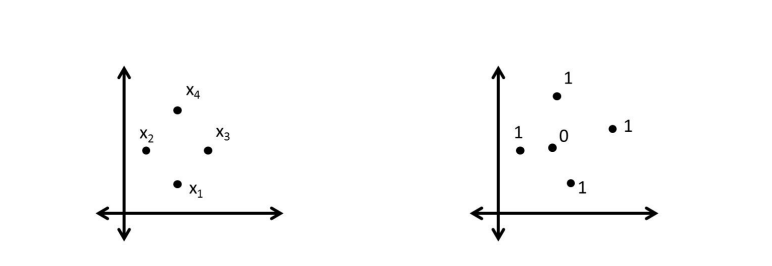
\includegraphics[width=\textwidth]{figures/vc_class_hypercubes_example.png}
    \caption{Example when $d=2$. Four points can be shattered by $\Hf$ but no five points can be shattered by $\Hf$.}
    \label{fig:vc_class_example_hypercubes}
\end{figure}

\noindent\newline\underline{\textbf{Example 2 } (Convex sets in $\R^2$)} : Let $\X=\R^2$. Consider the set of classifiers
\begin{align*}
    \Hf = \biggCurl{
        \1{x\in C} : C \text{ is convex in } \R^2
    }
\end{align*}

\noindent In this case, $V_\Hf=\infty$ because for any $n$ points on a circle and for any $1\le k \le n$, we can draw a polygon that includes $k$ points but not the remaining $n-k$ points for any selection of $k$ in $n$ points (Figure \ref{fig:vc_class_example_convexset}).
\begin{figure}[ht]
    \centering
    
\includegraphics[width=\textwidth]{figures/vc_class_convex_set_example.png}
    \caption{$\Hf$ can shatter any $n$ points on a circle.}
    \label{fig:vc_class_example_convexset}
\end{figure}

\noindent\newline\underline{\textbf{Example 3 } (Finite $|\Hf|$)} : For any function class where $|\Hf|<\infty$, we have:
\begin{align*}
    N_\Hf(x_1, \dots, x_n) &= \bigAbs{\bigCurl{
        (h(x_1), \dots, h(x_n)) : h \in \Hf
    }} \le |\Hf| \\
    \implies& S_\Hf(n) \le |\Hf| \\
    \implies& V_\Hf \le \log_2|\Hf|
\end{align*}

\begin{proposition}{Steele \& Dudley}{steele_dudley}
    Let $\F$ be the set of real-valued functions of the form:
    \begin{align*}
        \F = \bigCurl{
            f: \mathbb{R}^d \to \mathbb{R}
        }, \ dim(\F) = m
    \end{align*}
    \noindent Then, the following set of classifiers:
    \begin{align*}
        \Hf = \bigCurl{
            \1{f(x) \ge 0} : f \in \F
        }
    \end{align*}

    \noindent Has finite VC dimension. Specifically, $V_\Hf \le m$.
\end{proposition}

\begin{proof*}[Proposition \ref{prop:steele_dudley}]
    Suppose that $\Hf$ shatters $m+1$ points in $C=(x_1, \dots, x_{m+1})$. Define the linear mapping $L_C:\F \to \R^{m+1}$ such that:
    \begin{align*}
        L_C(f) = (f(x_1), \dots, f(x_{m+1}))^T
    \end{align*}

    \begin{subproof}{\newline Claim : $L_C(\F)$ is a closed subspace in $\R^{m+1}$}
        Let $\{l_n\}_{n=1}^\infty \subset L_C(\F)$ be a sequence and let $l_n\to l$ as $n\to\infty$. We can always choose a function $f\in\F$ such that:
        \begin{align*}
            f(x) = l, \ \forall x \in \mathbb{R}^m
        \end{align*}

        \noindent Hence, for all $\{l_n\}_{n=1}^\infty$ such that $l_n\to l$, the limit $l\in L_C(\F)$. Therefore, $L_C(\F)$ is closed in $\R^{m+1}$.
    \end{subproof}

    \noindent By the Hilbert Projection Theorem \cite{wiki:hilbert_projection_theorem}, we have:
    \begin{align*}
        \R^{m+1} = L_C(\F) \oplus L_C(\F)^\bot 
    \end{align*}

    \noindent Since $dim(\F)=m$, we have $dim(L_C(\F)) \le m$. Therefore, $dim(L_C(\F)^\bot) \ge 1$ and we have:
    \begin{align*}
        \forall f\in\F, \exists \gamma \in \R^{m+1}\setminus \{0\} : \gamma^TL(f) = 0 
    \end{align*}

    \noindent Equivalently,
    \begin{align*}
        \sum_{i=1}^{m+1}\gamma_i f(x_0) = 0 \implies \sum_{i, \gamma_i \ge 0} \gamma_if(x_i) = \sum_{j, \gamma_j < 0} -\gamma_j f(x_j)
    \end{align*}

    \noindent Since $\Hf$ shatters $x_1, \dots, x_{m+1}$. We define a classifier $h\in\Hf$ such that:
    \begin{align*}
        h(x_i) = \begin{cases}
            1 &\text{if } \gamma_i \ge 0 
            \\ \\
            0 &\text{otherwise}
        \end{cases} 
        \implies
        f(x_i) \ge 0 \iff \gamma_i \ge 0
    \end{align*}
    \noindent This implies that $\sum_{i:\gamma_i \ge 0}\gamma_if(x_i) \ge 0$ and $\sum_{j:\gamma_j < 0}-\gamma_j f(x_j) < 0$, which is a contradiction. Therefore, we have $V_\Hf<\infty$.
\end{proof*}

\begin{corollary}{Linear classifiers have finite $V_\Hf$}{linear_clf_has_finite_vcdim}
    Let $\X=\R^d$ and define a function space $\F$ as:
    \begin{align*}
        \F = \bigCurl{
            f:\R^d\to\R \Big| f(x) = w^Tx + b, \ w\in\R^d, b\in\R
        }
    \end{align*}

    \noindent Then, define the set of linear classifiers as:
    \begin{align*}
        \Hf = \bigCurl{
            \1{w^Tx+b\ge 0} \Big| w\in \R^d, b\in\R
        }
    \end{align*}

    \noindent We have $V_\Hf\le d+1$.
\end{corollary}

\begin{proof*}{Corollary \ref{coro:linear_clf_has_finite_vcdim}}
    Since $dim(\F)=d+1$, the above corollary is a direct consequence of proposition \ref{prop:steele_dudley}.
\end{proof*}


\subsection{VC Theorem for sets}
\begin{definition}[VC Theory for sets]
    Let $\mathcal{G}$ be a collection of subsets in $\X$. Let $C\subset\X$ and $C=\{x_1, \dots, x_n\}$. We have the following definitions for restriction of $\mathcal{G}$ to $C$, shattering coefficient and VC-dimension of $\mathcal{G}$:
    \begin{align*}
        N_\mathcal{G}(C) &= \bigAbs{ \bigCurl{ G \cap C : G \in \mathcal{G} } } \\
        S_\mathcal{G}(n) &= \sup_{C\subset\X; |C|=n} \bigAbs{ N_\mathcal{G}(C) } \\
        V_\mathcal{G}    &= \sup\bigCurl{ n : S_\mathcal{G}(n) = 2^n } = \sup_{C\subset\X}\bigCurl{ |C| : \mathcal{G} \text{ shatters } C }
    \end{align*}
\end{definition}

\textbf{Remark} : In analogy to the definitions for classifier, sets and binary classifiers are equivalent via:
\begin{align*}
    G &\to h_G(x) = \1{x \in G} \\
    h &\to G_h = \bigCurl{ x : h(x)=1 }
\end{align*}

\begin{theorem}{VC Theorem (for sets)}{vc_theorem_for_sets}
    If $X_1, \dots, X_n\sim Q$ are identically independently distributed samples. Then for any collection $\mathcal{G}$ of subsets in $\X$, $\epsilon>0$, we have:
    \begin{align*}
        P\biggRound{
            \sup_{G\in\mathcal{G}} \bigAbs{
                \widehat{Q}(G) - Q(G) 
            }\ge \epsilon
        } \le 8S_\mathcal{G}(n)e^{-n\epsilon^2/32}
    \end{align*}

    \noindent Where $\widehat{Q}(G)$ is defined (similar to the empirical CDF) as:
    \begin{align*}
        \widehat{Q}(G) = \frac{1}{n}\sum_{i=1}^n \1{X_1\in G}
    \end{align*}
\end{theorem}

\begin{proof*}[Theorem \ref{thm:vc_theorem_for_sets}]
    Define the following class of classifiers:
    \begin{align*}
        \Hf = \bigCurl{
            h_G = \1{x\in G} : G \in \mathcal{G}
        }
    \end{align*}

    \noindent Define a density function over $\X\times\{0,1\}$ such that $\pi_0=1$, $P_{X|Y=0}=Q$ and $P_{X|Y=1}$ is arbitrary. For any $h_G\in \Hf$, we have:
    \begin{align*}
        R(h) &= P(h_G(X) \ne Y) \\
        &= \pi_0P_{X|Y=0}(h_G(X) \ne 0) + \pi_1 P_{X|Y=1}(h_G(X) \ne 1) \\
        &= \pi_0P_{X|Y=0}(h_G(X) = 1) + \pi_1 P_{X|Y=1}(h_G(X) = 0) \\
        &= P_{X|Y=0}(h_G(X) = 1) \ \ \ (\text{Since } \pi_0=1, \pi_1=0)\\
        &= Q(G)
    \end{align*}

    \noindent Similarly, we have:
    \begin{align*}
        \widehat{R_n}(h_G) = \frac{1}{n}\sum_{i=1}^n \1{h_G(X_i) = 1} = \frac{1}{n}\sum_{i=1}^n \1{X_i\in G} = \widehat{Q}(G)
    \end{align*}

    \noindent Therefore:
    \begin{align*}
        P\biggRound{
            \sup_{G\in\mathcal{G}} \bigAbs{
                \widehat{Q}(G) - Q(G) 
            }\ge \epsilon
        }
        &= 
        P\biggRound{
            \sup_{h_G\in\mathcal{H}} \bigAbs{
                \widehat{R_n}(h_G) - R(h_G) 
            }\ge \epsilon
        } \\
        &\le 8S_\Hf(n)e^{-n\epsilon^2/32} \ \ \ (\text{Theorem }\ref{thm:udb_non_finite_h}) \\
        &= 8S_\mathcal{G}(n)e^{-n\epsilon^2/32}
    \end{align*}
\end{proof*}

